\section{Mixture Models} \label{mixture-models-section}

The aim of this project is focused on modelling and clustering multisource biomedical data. Clustering is a widely used exploratory tool, whose main task is to identify and group similar objects together in \emph{'clusters'}. Clustering can can be categorized as an \emph{unsupervised} learning approach, since we try to discover hidden structure in unlabelled data.     

Different algorithms have been proposed for performing clustering, including hierarchical clustering (agglomerative or top down), k-means \citep{MacQueen1967}, and mixture models \citep{McLachlan1988}. This project is concentrated on \emph{mixture models} which are probabilistic, in the sense that they claim how the data might look like by modelling each cluster by certain probability density functions, \eg mixture of Gaussian distributions.  

A mixture model is a convex combination of two or more probability density functions, possibly of different distributional types. By using a superposition of the individual probability density functions, mixture models are capable of approximating any continuous distribution to arbitrary accuracy \citep{Marin2005}. Mixture models can be formulated as Latent Variable Models (LVMs), where the latent variables have discrete states and can be interpreted as defining assignments of data points to specific components of the mixture model.

Formally, let $x_{i}$, where $i \in \lbrace 1, ... , N \rbrace$, be a given dataset with N objects. The goal of clustering is to partition the objects into at most K clusters. Let $p(x_{i}|\theta)$ be the probability distribution for $x_{i}$ parametrized by $\theta$, $z_{i} \in \lbrace 1,...,K \rbrace$ represent the component that is responsible for $x_{i}$, and $\pi_{k}$ be the probability that an object belongs to cluster $k$, \ie $\pi_{k} = p(z_{i} = k)$. We refer to $\pi_{k}$ as \emph{mixing proportions} and to $z_{i}$ as \emph{latent variables} since they are not observed in the data, but are introduced to allow complicated distributions to be formed from simpler components. 

Thus, the mixture model is defined as follows:
\begin{equation} \label{mix-model-f-mm}
	\begin{aligned}
		p(x_{i}|\Theta) & = \sum_{k=1}^{K} p(z_{i} = k) p(x_{i}|\theta_{k}) \\
			& = \sum_{k=1}^{K}\pi_{k} p(x_{i}|\theta_{k})
	\end{aligned}
\end{equation}
where $\Theta = (\theta_{1},..., \theta_{k}, \pi_{1},..., \pi_{k})$ is the set of all parameters, which must satisfy:
\begin{equation}
		\pi_{k} \in (0, 1) \; \text{for} \; k \in \lbrace 1,...,K \rbrace, \; and 
\end{equation}
\begin{equation}
		\sum_{k=1}^{K}\pi_{k} = 1 
\end{equation}

Mixture models are \emph{generative models}, which means that they give us information for generating new objects. The procedure is the following: first we choose a component, with probabilities given by the mixing proportions, and then we generate an object from the corresponding probability distribution. Formally:
\begin{equation}
	\begin{aligned}
		z_{i} \; & \sim \; Cat(\pi_{1},...,\pi_{K}) \\
		x_{i} | z_{i}=k \; & \sim \; p(x_{i}|\theta_{k})
	\end{aligned}
\end{equation}
where $Cat(\pi_{1},...,\pi_{K})$ is the \emph{categorical} distribution, \ie \emph{multinomial} distribution over a single trial.

\emph{Fig.\ref{gmm-pic}} shows a Gaussian Mixture Model (GMM) with three components in two-dimensional space. It is clear that a single Gaussian distribution would be unable to capture the characteristics of the data since it is unimodal, but a linear superposition of $K$ Gaussian distributions can approximate the continuous density of the data to arbitrary accuracy. 

\begin{figure}[!ht]
	\begin{center}
 		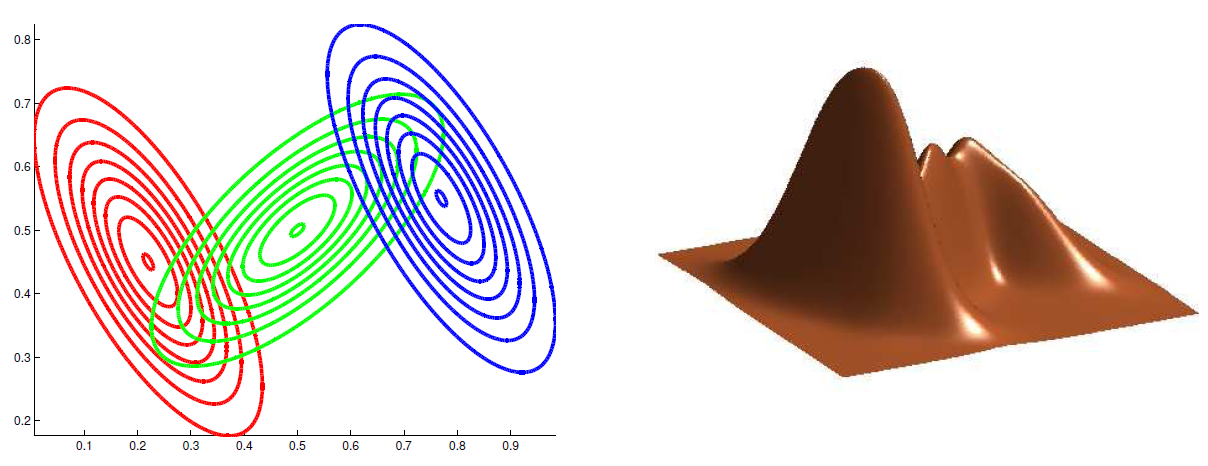
\includegraphics[scale = 0.43]{images/gmm.png}
		 	  \caption{\emph{\textbf{Left:} Contours of constant density for each of the mixture components, where each component is denoted by a different colour. \textbf{Right:} A surface plot of the probability distribution $p(\mathbf{X}|\Theta)$ \cite[Ch. \ 2]{Bishop2006}.}}
		\label{gmm-pic}
	\end{center}
\end{figure}

\subsection{Mixture Model Estimation} \label{mixt-model-estimation-l-subsect}
The model can be fitted to the data using Maximum Likelihood Estimation (MLE). The likelihood is the probability of observing the data given the parameters, and is a function of the parameters. Given a dataset $\mathbf{X}$ consisting of $N$ independent and identically distributed (i.i.d) objects $x_{1}, ..., x_{N}$, the log likelihood function for any mixture model is given by:
\begin{equation} \label{likelihood-f-mm}
	\ell(\Theta) \triangleq p(\mathbf{X}|\Theta) = \sum_{i=1}^{N} \log \bigg\lbrace \sum_{k=1}^{K}\pi_{k}p(x_{i}|\theta_{k})\bigg\rbrace
\end{equation}
The MLE approach is to find the set of parameters $\Theta$ that maximizes \emph{Eq. \ref{likelihood-f-mm}}, that is:
\begin{equation} \label{MLE-f-mm}
	\hat{\Theta} =  \underset{\Theta}{\operatorname{argmax}} \; \ell(\Theta)
\end{equation}

Unfortunately, the presence of the summation inside the logarithm in \emph{Eq. \ref{likelihood-f-mm}} prevents the possibility of deriving an analytical solution. Thus, one should use numerical optimisation procedures, and one of the most widely used algorithms for estimating parameters of mixture models is \emph{Expectation Maximization} (EM) algorithm \citep{Dempster1977}. 
\subsection{The EM algorithm} \label{em-algorithm-l-subsect}
EM is a general iterative algorithm for computing MLEs when there are missing data or latent variables. As aforementioned, mixture models can be formulated as LVMs, thus, EM arises naturally and alternates between inferring the latent values given the parameters (\emph{E-step}), and then optimizing the parameters given the filled in data (\emph{M-step}). EM exploits the fact that if the data were fully observed then the MLE would be easy to compute. In their classic paper \cite{Dempster1977} proved that EM monotonically increases the log likelihood and it converges to a maximum likelihood estimator. The algorithm ends when a convergence criterion is satisfied, \eg the log likelihood does not increase above a certain threshold between two consecutive iterations. 

\emph{Fig. \ref{em-algorithm-pic}} illustrates the EM algorithm for the mixture of two Gaussian distributions applied to the Old Faithful dataset.
\begin{figure}[ht!]
     \begin{center}
        \subfigure[]{
            \label{fig:first}
            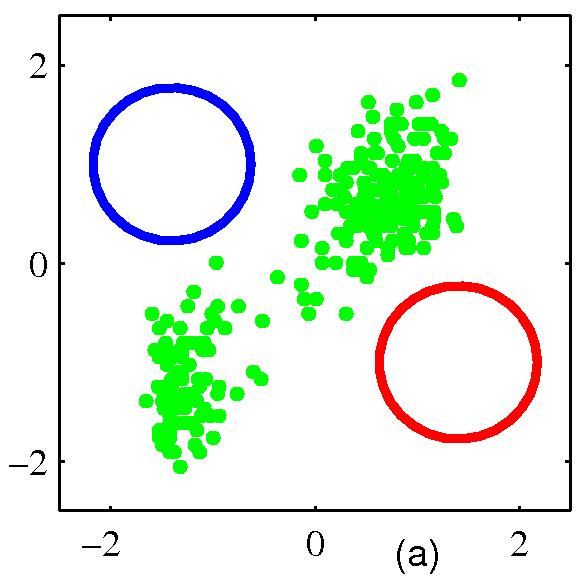
\includegraphics[width=0.3\textwidth]{images/em-a.jpg}
        }
        \subfigure[]{
           \label{fig:second}
           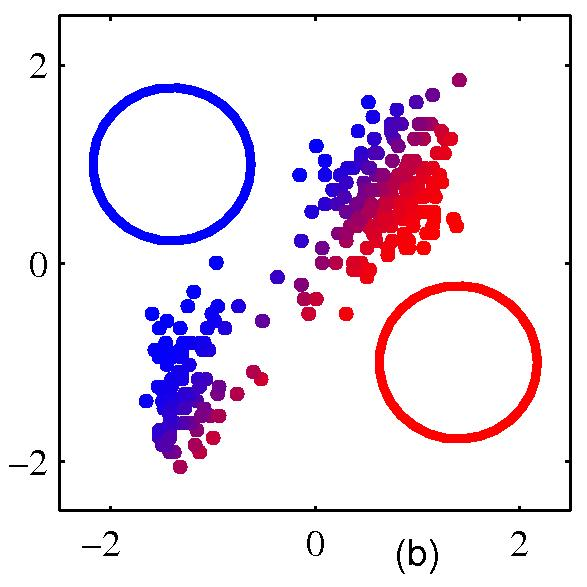
\includegraphics[width=0.3\textwidth]{images/em-b.jpg}
        }
        \subfigure[]{
            \label{fig:third}
            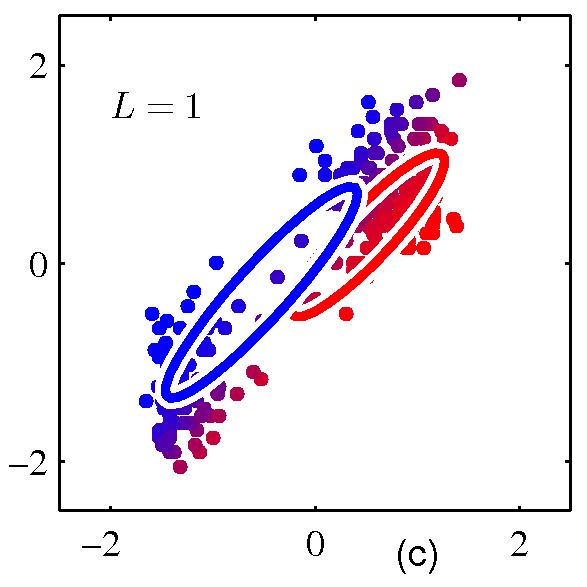
\includegraphics[width=0.3\textwidth]{images/em-c.jpg}
        } %  ------- End of the first row ----------------------%
        \subfigure[]{
            \label{fig:fourth}
            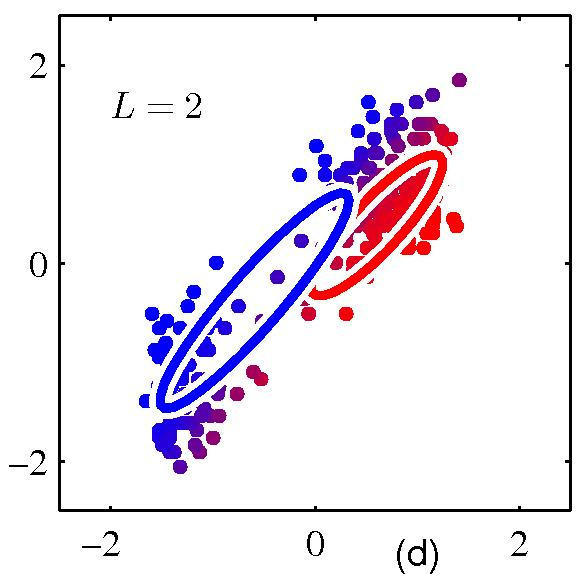
\includegraphics[width=0.3\textwidth]{images/em-d.jpg}
        }
        \subfigure[]{
            \label{fig:fifth}
            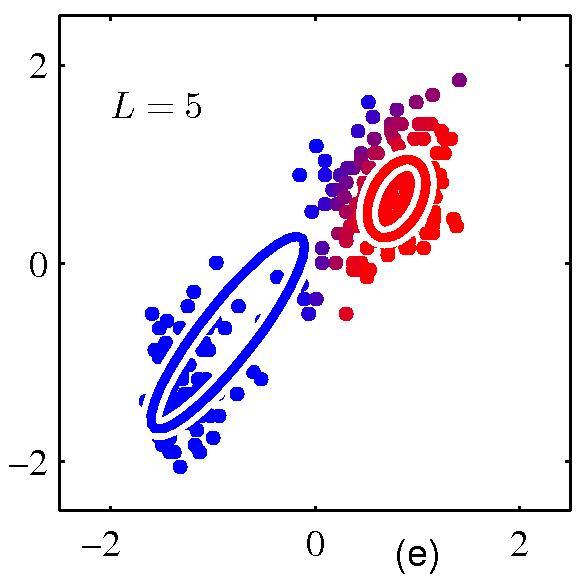
\includegraphics[width=0.3\textwidth]{images/em-e.jpg}
        }
        \subfigure[]{
            \label{fig:sixth}
            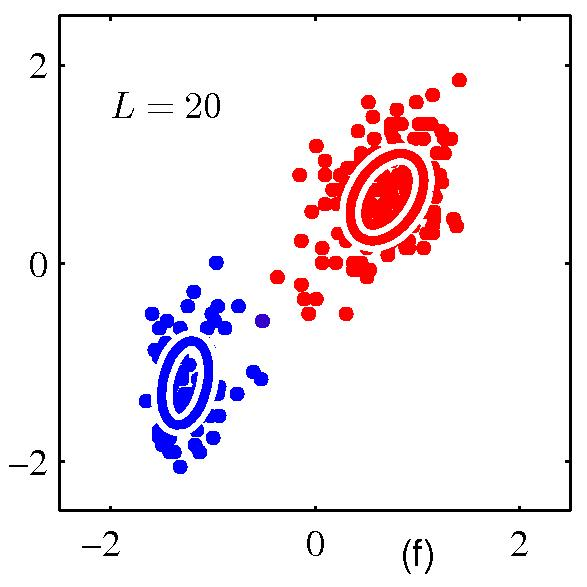
\includegraphics[width=0.3\textwidth]{images/em-f.jpg}
        }
    \end{center}
    \caption{\emph{Illustration of the EM algorithm using the Old Faithful dataset. Plot (a) shows initial parameters. Plots (b) and (c) show the E and M steps in the first iteration, respectively. Plots (d), (e) and (f) show the results after 2, 5 and 20 complete iterations of EM algorithm, respectively. \cite[Ch. \ 9]{Bishop2006}.}}
   \label{em-algorithm-pic}
\end{figure}

Our presentation for the derivation of the EM algorithm is based on \cite[Ch. \ 11]{Murphy2012}.

Let $x_{i}$ be the observed variables, and $z_{i}$ be the hidden or latent variables. We are interested in maximizing the log likelihood of the observed data:
\begin{equation} \label{log-lik-observed-f-mm}
	\ell(\Theta) \triangleq \sum_{i=1}^{N} \log p(x_{i}|\theta) =  \sum_{i=1}^{N} \log \bigg[\sum_{z_{i}} p(x_{i}, z_{i}|\theta) \bigg]
\end{equation}
which is hard to optimize due to the presence of the summation inside the logarithm, so the logarithm no longer acts directly on the likelihood function.

Let us define the \emph{complete data log likelihood} as follows:
\begin{equation} \label{log-lik-comp-observed-f-mm}
	\ell_{c}(\Theta) \triangleq \sum_{i=1}^{N} \log p(x_{i}, z_{i}|\theta)
\end{equation}

If the variables $z_{i}$ were observed, we assume that this likelihood could be easily computed. EM gets around this problem by defining the \emph{expected complete data log likelihood} as:
\begin{equation} \label{log-lik-expected-f-mm}
		Q(\Theta, \Theta^{t-1}) \triangleq \mathbb{E} \big[\ell_{c}(\Theta) | \mathbf{X}, \Theta^{t-1}\big]
\end{equation}
where $t$ is the current iteration. The expectation is taken with respect to the old parameters $\Theta^{t-1}$ and the observed data $\mathbf{X}$. In the \emph{E-step}, we compute the terms inside $Q(\Theta, \Theta^{t-1})$ for which MLE depends on. In the \emph{M-step}, we optimize Q w.r.t $\Theta$:
\begin{equation} \label{max-log-lik-observed-f-mm}
	\Theta^{t} = \underset{\Theta}{\operatorname{argmax}} \; Q(\Theta, \Theta^{t-1})
\end{equation}

For the specific case of mixture models, the expected complete data log likelihood is:
\begin{equation} \label{log-lik-expected-derivation-f-mm}
	\begin{aligned}
		Q(\Theta, \Theta^{t-1}) & \triangleq \mathbb{E} \big[\ell_{c}(\Theta) | \mathbf{X}, \Theta^{t-1}\big] \\
								& = \mathbb{E} \bigg[ \sum_{i} \log p(x_{i}, z_{i}|\theta) \bigg] \\
								& = \sum_{i} \mathbb{E} \bigg[ \log \bigg[\prod_{k} \big( \pi_{k}p(x_{i}|\theta_{k})\big)^{\mathbb{I}(z_{i}=k)} \bigg]\bigg] \\
								& = \sum_{i} \sum_{k} \mathbb{E} \big[\mathbb{I}(z_{i}=k)\big] \log \big[\pi_{k}p(x_{i}|\theta_{k})\big] \\
								& = \sum_{i} \sum_{k} p(z_{i}=k|x_{i},\theta_{k}^{t-1}) \log \big[\pi_{k}p(x_{i}|\theta_{k})\big] \\
								& = \sum_{i} \sum_{k} \gamma(z_{ik}) \log \big[\pi_{k}p(x_{i}|\theta_{k})\big] \\
								& = \sum_{i} \sum_{k} \gamma(z_{ik}) \log \pi_{k} + \sum_{i} \sum_{k} \gamma(z_{ik}) \log p(x_{i}|\theta_{k}) \\		
	\end{aligned}
\end{equation}
where, $\gamma(z_{ik}) \triangleq p(z_{i}=k|x_{i},\theta_{k}^{t-1})$ is the responsibility that component k takes for explaining the observation $x_{i}$, and $\mathbb{I}(z_{i}=k)$ is an indicator function, equal to 1 if $z_{i}=k$, and 0 otherwise.


\subsubsection{E-Step}
The E-step can be computed using the following form for any mixture model, which is the responsibility that component k takes for explaining the observation $x_{i}$:
\begin{equation} \label{responsibilities-f-mm}
  \begin{aligned}
	\gamma(z_{ik}) & \triangleq p(z_{i}=k|x_{i},\theta_{k}^{t-1}) \\
				   & = \frac{p(z_{i}=k)p(x_{i}|z_{i}=k,\theta_{k}^{t-1})}{\sum\limits_{j=1}^{K} p(z_{i}=j)p(x_{i}|z_{i}=j,\theta_{j}^{t-1})} \\
				   & = \frac{\pi_{k}p(x_{i}|z_{i}=k,\theta_{k}^{t-1})}{\sum\limits_{j=1}^{K} \pi_{j}p(x_{i}|z_{i}=j,\theta_{j}^{t-1})}
  \end{aligned}
\end{equation}


\subsubsection{M-Step}
In the M-step we optimize $Q$ with respect to parameters $\Theta = (\theta_{1},...,\theta_{K},\pi_{1},...,\pi_{K})$.

For the mixing proportions $\pi_{k}$, we take the derivative of \emph{Eq. \ref{log-lik-expected-derivation-f-mm}} w.r.t. $\pi_{k}$ and set it to zero; due to the constraint that $\sum_{k=1}^{K}\pi_{k} = 1$ we introduce a Lagrange multiplier. Thus we have:

\begin{equation} \label{derivative-mix-prop-f-mm}
  \begin{aligned}
	\frac{\partial}{\partial \pi_{k}} \bigg[  Q(\Theta, \Theta^{t-1}) + \lambda \big( \sum_{k}\pi_{k} - 1\big) \bigg] & = 0 \\
	\sum_{i} \frac{1}{\pi_{k}} \gamma(z_{ik}) + \lambda & = 0 
  \end{aligned}
\end{equation}
Setting $\lambda = - N$, the result, which is the same for any mixture model, is:
\begin{equation} \label{mixing-proportions-est-f-mm}
		\pi_{k} = \frac{1}{N} \sum_{i} \gamma(z_{ik})
\end{equation}

To derive the M-step for the parameters $\theta_{k}$, we only need to keep the terms of \emph{Eq. \ref{log-lik-expected-derivation-f-mm}} that depend on $\theta_{k}$, that is:
\begin{equation} \label{parameters-est-EM-M-f-mm}
		\ell(\theta_{k}) \triangleq \sum_{i} \sum_{k} \gamma(z_{ik}) \log p(x_{i}|\theta_{k})
\end{equation}
and we optimize them with respect to $\theta_{k}$.

The maximization of \emph{Eq. \ref{parameters-est-EM-M-f-mm}} yields different results depending on the probability distribution $p(x_{i}|\theta_{k})$. For most of the well known probability distributions, including the Normal, Binomial, Poisson, etc., direct maximization of $\ell(\theta_{k})$ is feasible. 

For more complex likelihood functions, the maximization of $\ell(\theta_{k})$ may be intractable, thus numerical optimization strategies \citep{Nocedal2006}, such as conjugate gradients algorithm \citep{Hestenes1952} should be exploited. This extension of EM algorithm is known as \emph{Generalised EM}, or GEM, and it has been proved that on each EM iteration of the GEM algorithm the log likelihood increases, and thus converges to the maximum likelihood estimate \citep{Wu1983}.